\section{Reducing the computational overhead}

% integral image
During the shift from the initial tests involving the usage of labeled bounding boxes to the actual requirement of finding parts inside of image databases, the amount of computational overhead increased significantly as it requires to compute sliding windows on each image in the database and their codebooks respectively.

Therefore the idea came up to precompute the codebooks and only load them at runtime for comparison. One solution would be to compute a set of possible windows and their codebooks. At query time the best matching window ratios could be loaded and compared to the query codebook. Unfortunately the performance was dramatically decreased with this approach.

The second solution was to create integral images based on codebooks. Integral images were described by Viola and Jones in 2001 \cite{viola2001rapid}. Such images are created by summing up all pixel values from the top left to the bottom right (or any other diagonal direction). The advantage of this approach is the possibility to compute a sum value for a rectangular area by summing and subtracting the values of the four corners as described in \figref{integral_image}. 

\begin{figure}
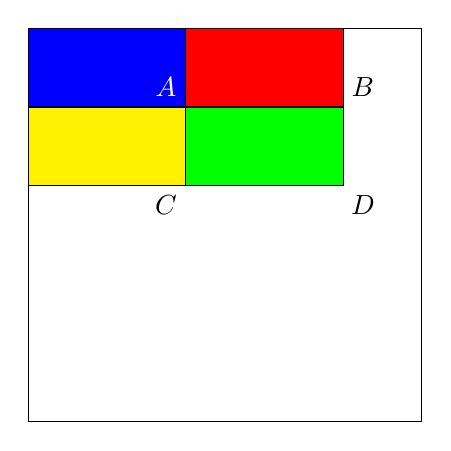
\begin{tikzpicture}
\draw (0,0) rectangle (5,5);
\draw[fill=blue] (0,5) rectangle (2,4);
\draw (1.75, 4.25)  node[white] {$A$};
\draw[fill=red] (2,5) rectangle (4,4);
\draw (4.25, 4.25)  node{$B$};
\draw[fill=yellow] (0,4) rectangle (2,3);
\draw (1.75, 2.75)  node{$C$};
\draw[fill=green] (2,4) rectangle (4,3);
\draw (4.25, 2.75)  node{$D$};
\end{tikzpicture}
\caption[Sum of area in integral image]{The sum of all values in the green area could be computed by $A+D-(C+B)$. $A$ is the sum of all pixels in the blue area, $B$ the sum of the pixels in the blue and the red areas, $C$ the sum of all pixels in the blue and yellow areas, $D$ of the green, red, blue and yellow respectively}
\label{fig:integral_image}
\end{figure}

The difference to \cite{viola2001rapid} is that one pixel at a time is represented by a complete codebook, therefore an integral image per codebook dimension has to be computed. The source image is created by adding the inverse distance of each feature patch center to its nearest cluster centroid to the corresponding codebook dimension. Afterwards, a cumulative sum over the two image axes is computed. The benefit of using integral images is that at runtime, every possible window could be computed by four reads (the corners), one sum and two subtractions between the codebooks. This reduced the computational time at the query stage to 1-2 seconds with a $500\times375$ image, 1000 codebook dimensions and 5000 windows with a 2-by-2 grid.

The downside is the memory usage, which increased dramatically. For example, a $500 \times 375 \times 1000$ integral image requires with the double datatype at least 1.4 gigabytes of data (without any meta information stored aside by matlab). The 50 images test database required therefore at least 70 gigabytes of RAM storage during the query. This also led to the problem of the time required to load the whole database. By storing it in the \MATLAB 7.3 file format, which effectively is a slightly modified HDF5 \cite{hdf5}, the program requires in average 900 seconds to load the whole database from a network shared filesystem.

This method also enabled the extraction of the query codebook from an image contained in the database without any feature or codebook computations. The reduced computational effort during the query phase consist therefore in extracting the query codebook from the database, training of the \ac{SVM}, calculating the sliding windows, extracting the codebook for each window in each image and scoring the codebooks by the trained \ac{SVM}.

Further tests showed that the performance was highly related to the size of the query image part. The assumption based on this observations was that the smaller feature patches created to much background clutter and therefore obscure the main information in high resolution images. Most of the current part retrieval algorithms overcome this problem by rescaling the image for the different window sizes. As all information about the original patches got lost during the conversion into the integral images, there is no way to filter the extracted codebooks to remove the additional information from smaller or bigger patches.

To solve this problem, multiple scale ranges were introduced. For each image a list of included scales from the feature pyramid was build during the generation of the image database. The list is split into multiple parts of the same length. Each of this parts denotes a range of scales which are included in the resulting integral image. If for example during the creation of the database an amount of three scale ranges was configured, there will be three files for each image processed and three different image databases created. The filenames contain the maximum size of the contained feature patches in pixels (for example $86 \times 86$).

During the query step, the size of the query image part is taken and the database with the best matching scales will be loaded. The selection is done by requiring a minimum amount of possible features inside the extracted windows. If for example a requirement of at least two features per window dimension is required and the query image part has an width of 200 pixels, the image database loaded should not have patches included with more than 100 pixels in width.

By using this separation the amount of false positives decreased as the windows become more comparable to the query image part. It should be noted that even as the amount of feature patches involved during the integral image decreased, the memory usage stays the same as only the codebook values are affected by the lesser information. Nevertheless, it does affect the memory optimizations done in \prettyref{sec:reducing_memory} as much more codebook entries are filled with null values.
% no libsvm classify